% !TeX root = main.tex

\section{Q3: Bounding Box}

\paragraph*{Question}
\begin{displayquote}
    % Contents of question 3
You've been provided with an image taken from a self-driving car that shows another car in front. A camera has been placed on top of the car, 1.65 m from the ground. The camera intrinsic matrix $K$ is provided.
Your task is to draw a 3D-bounding box around the car in front. Your approach should be to place eight points in the 3D world such that they surround all the corners of the car, then project them onto the image and connect the projected image points using lines. Make a python program for this.

Assume that the image plane is perfectly perpendicular to the ground.
You might have to apply a small 5° rotation about the vertical axis to align the box perfectly. 
Rough car dimensions - h: 1.38 m, w: 1.51, l: 4.10.
Also, estimate the approximate translation vector to the mid-point of the two rear wheels of the car in the camera frame.

\end{displayquote}

The image given is

\begin{figure}[h]
    \centering
    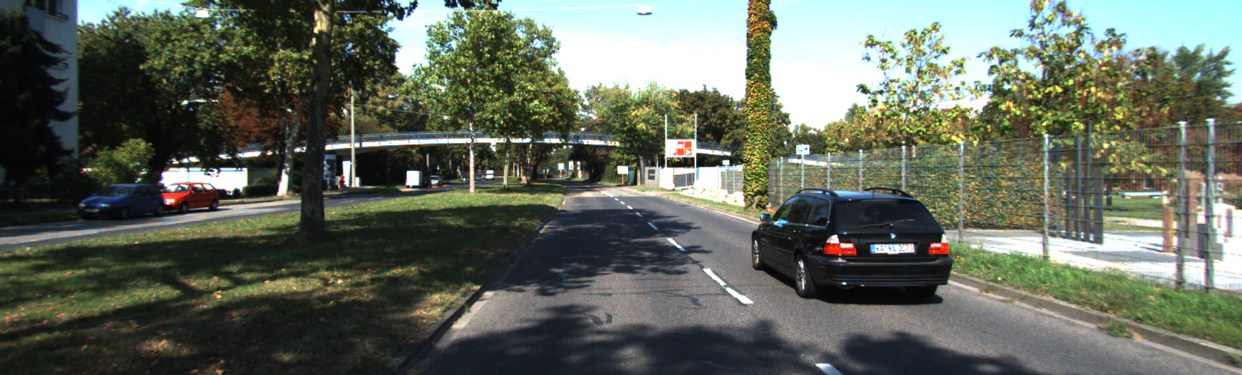
\includegraphics[width=0.9\textwidth]{bounding_box_vehicle_img.png}
\end{figure}

The camera projection matrix is

\begin{displayquote}
    K = [7.2153e+02,0,6.0955e+02;0,7.2153e+02,1.7285e+02;0,0,1]
\end{displayquote}

\subsection{Theory}

For the context, refer to the image below

\begin{figure}[h]
    \centering
    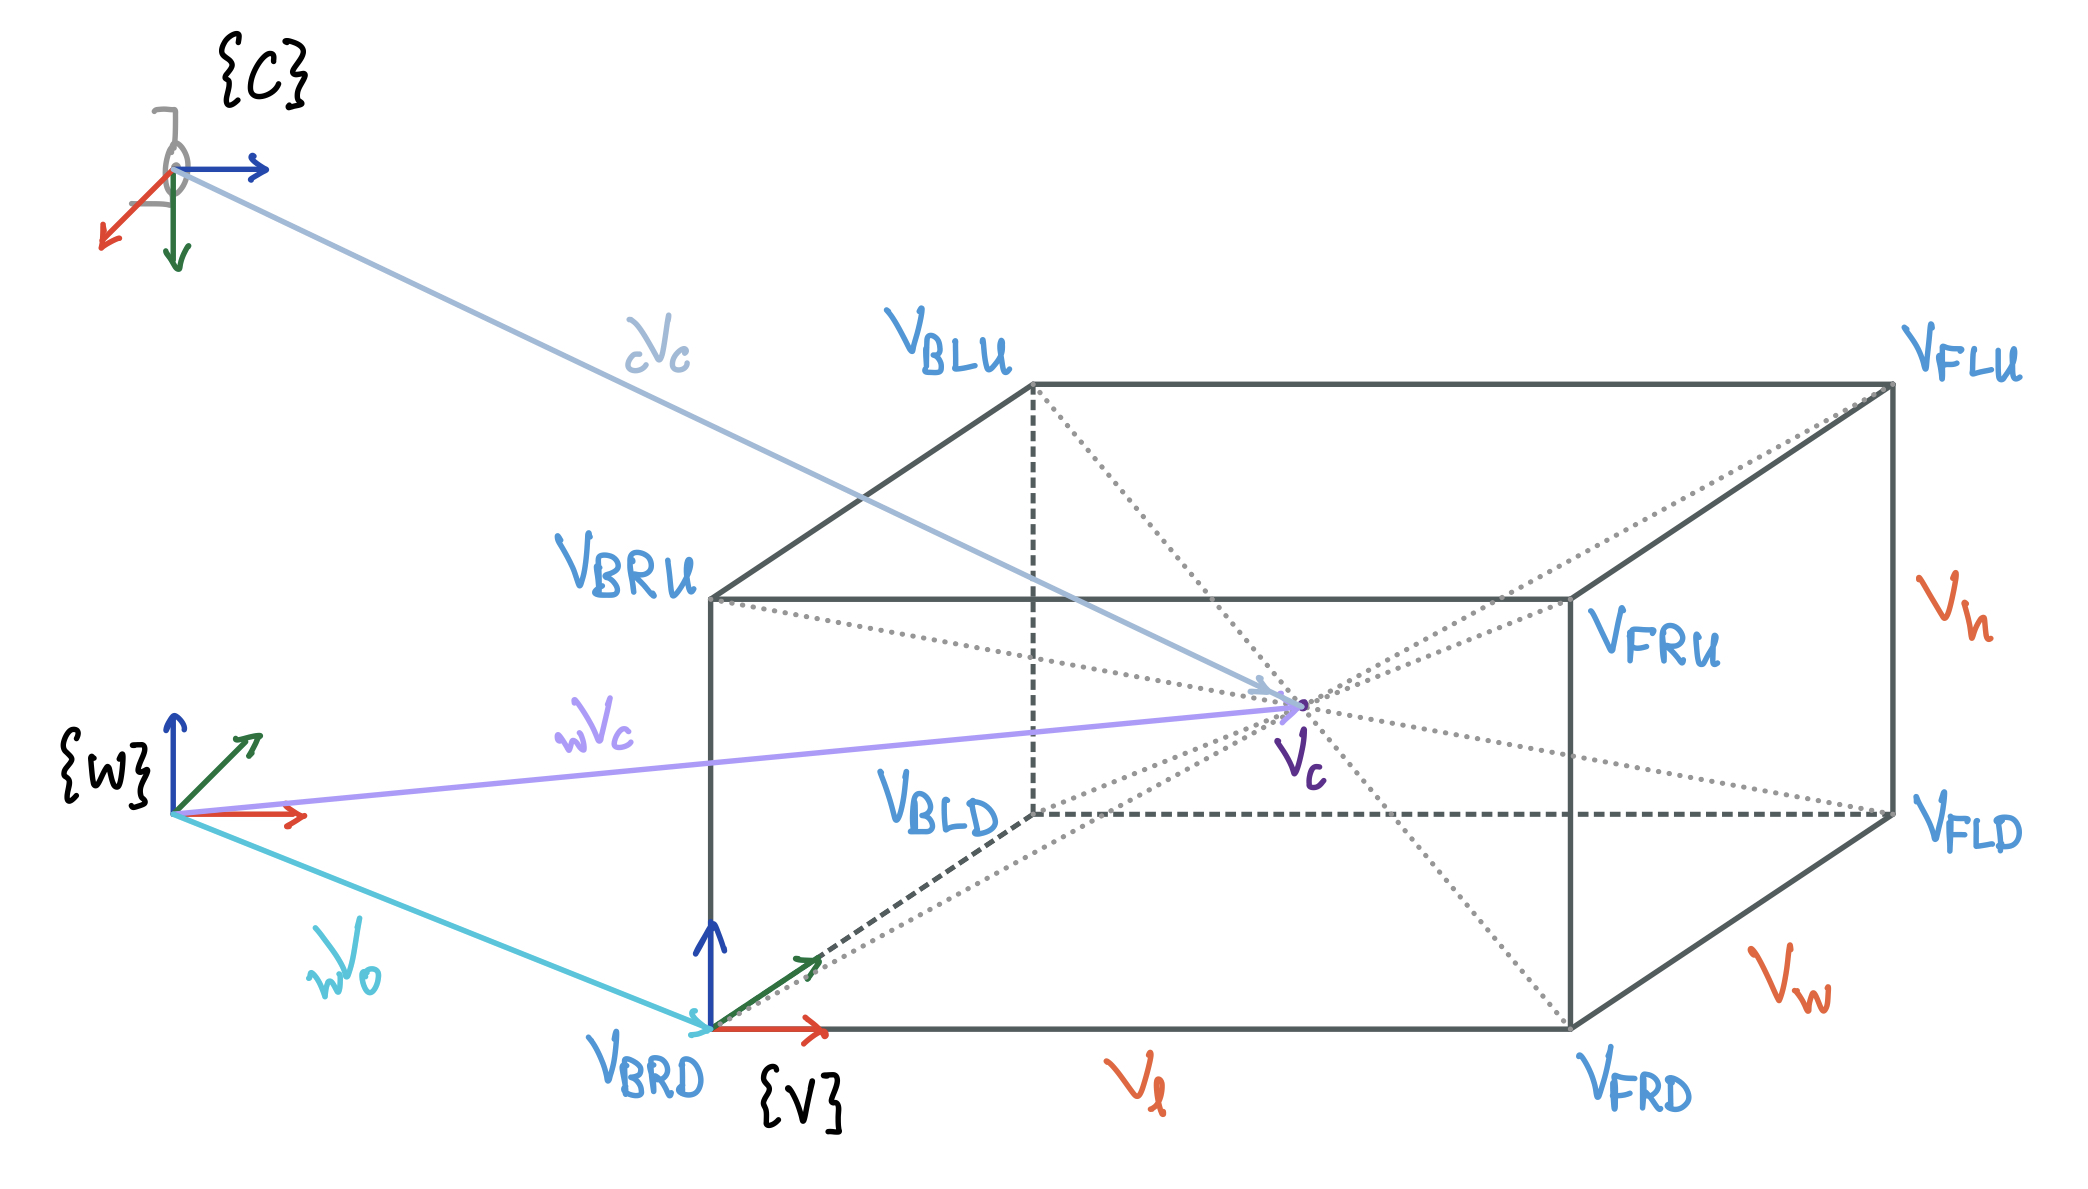
\includegraphics[width=0.7\textwidth]{bounding_box_theory_model.PNG}
    \caption{System Model}
    \label{fig:q3-model}
\end{figure}

\paragraph*{Frames}
The following frames are described in the figure \ref{fig:q3-model}

\begin{itemize}
    \item \textbf{World frame} $\{\textrm{W}\}$: The frame directly below the camera, fixed to the vehicle. This frame could be the odometry frame (whose transform to all sensors on the vehicle is known).
    \item \textbf{Vehicle frame} $\{\textrm{V}\}$: The vehicle frame. This is attached to the \textit{rear bottom right} of the vehicle, which is being localized.
    \item \textbf{Camera frame} $\{\textrm{C}\}$: The camera frame. The Z-axis looks out, Y goes down, and X to the right. It is assumed that the transform between this and the world frame $\{\textrm{W}\}$ is known.
\end{itemize}

\paragraph*{Vectors}

The following vectors are important

\begin{itemize}
    \item The vector $_{\textrm{W}}\textup{V}_{\textup{O}}$ is the point $\textup{V}_{\textup{BRD}}$ represented in $\{\textrm{W}\}$
    \item The vector $_{\textrm{V}}\textup{V}_{\textup{C}}$ is the vector of the centroid of the bounding box in $\{\textrm{V}\}$. This is not shown above, but is implicitly assumed. The vectors $_{\textrm{W}}\textup{V}_{\textup{C}}$ and $_{\textrm{C}}\textup{V}_{\textup{C}}$ are the projections (transforms) of this vector in $\{\textrm{W}\}$ and $\{\textrm{C}\}$ respectively.
    \item The vector $_{\textrm{W}}\textup{C}_{\textup{O}}$ is the origin of $\{\textrm{C}\}$ expressed in $\{\textrm{W}\}$
\end{itemize}

\paragraph*{Symbols}

The following symbols are used in the derivation hereon

\begin{itemize}
    \item $v_x$ and $v_y$ are the X and Y coordinates of $_{\textrm{W}}\textup{V}_{\textup{O}}$ (the Z coordinate is 0). These have to be computed (they are unknowns).

    \item $v'_{cx}$ and $v'_{cy}$ are the \emph{pixel coordinates} (X and Y) of the image of $_{\textrm{C}}\textup{V}_{\textup{C}}$ in the camera.
    
    The user can pick this, but it can also be retrieved through a detection algorithm (through the center of bounding boxes, maybe). These are, therefore, known.

    \item $v_l$, $v_w$, and $v_h$ are the length, width, and height of the bounding box of the vehicle (in the real world measurements). These are known.

    \item $V_\theta$ or $v_\theta$ is the yaw (rotation about Z in radians) of $\{\textrm{V}\}$ in $\{\textrm{W}\}$. This is also given in the statement.

    \item $C_h$ is the height of the camera above ground
\end{itemize}

\paragraph*{Important Notes}

The following points are important

\begin{itemize}
    \item The edges/corners of the bounding box are in blue. Each corner is named (subscript) according to position on X-axis (\texttt{B}ack or \texttt{F}ront), followed by position on Y-axis (\texttt{L}eft or \texttt{R}ight) followed by position on Z axis (\texttt{U}p or \texttt{D}own).

    These axes are of $\{\textrm{V}\}$, and the points are the 3D corners of the bounding box. The origin of $\{\textrm{V}\}$ is at $\textup{V}_{\textup{BRD}}$, and the problem entails finding this point in the XY plane of $\{\textrm{W}\}$. If we find this, we can automatically find every other point on the vehicle (they're all rigid).

    \item The point $\textup{V}_{\textup{C}}$ is the centroid of the vehicle (in front). A nice property of projection homography (transform) is that it \emph{preserves line intersections}. The centroid is the intersection of 4 lines (body diagonals of the cuboid).
    
    Usually, we have an object detection algorithm that gives us the \emph{bounding box} of the car ahead (which is a rectangle in pixel coordinates). The center of this bounding box can be projected outwards (as a line, if we know the camera intrinsic matrix $\mathbf{K}$) to intersect with the actual center of the cuboid (described by points above). This is a \textbf{critical} assumption of this method.
\end{itemize}

\subsubsection{Theoretical Solution}

With respect to $\{\textrm{V}\}$ and $\{\textrm{W}\}$, we know the following

\begin{align*}
    _{\textrm{V}}\textup{V}_{\textup{O}} = \begin{bmatrix}
    0 \\ 0 \\ 0 \\ 1
    \end{bmatrix}
    &&
    _{\textrm{W}}\textup{V}_{\textup{O}} = \begin{bmatrix}
    v_x \\ v_y \\ 0 \\ 1
    \end{bmatrix}
    &&
    _{\textrm{V}}\textup{V}_{\textup{C}} = \begin{bmatrix}
    v_l/2 \\ v_w/2 \\ v_h/2 \\ 1
    \end{bmatrix}
    &&
    ^{\textrm{W}}_{\textrm{V}}\mathbf{T} = \begin{bmatrix}
    \cos(v_\theta) & -\sin(v_\theta) & 0 & v_x \\
    \sin(v_\theta) & \cos(v_\theta) & 0 & v_y \\
    0 & 0 & 1 & 0 \\
    0 & 0 & 0 & 1
    \end{bmatrix}
\end{align*}

\begin{align*}
    \rightarrow \;
    _{\textrm{W}}\textup{V}_{\textup{C}} = \; ^{\textrm{W}}_{\textrm{V}}\mathbf{T} \; _{\textrm{V}}\textup{V}_{\textup{C}}
\end{align*}

With respect to $\{\textrm{C}\}$ and $\{\textrm{W}\}$, we know the following

\begin{align*}
    _{\textrm{W}}\textup{C}_{\textup{O}} = \left[\begin{matrix}0\\0\\C_{h}\\1\end{matrix}\right] &&
    ^{\textrm{W}}_{\textrm{C}}\mathbf{T} = \left[\begin{matrix}0 & 0 & 1 & 0\\-1 & 0 & 0 & 0\\0 & -1 & 0 & C_{h}\\0 & 0 & 0 & 1\end{matrix}\right]
    \rightarrow \; 
    ^{\textrm{C}}_{\textrm{W}}\mathbf{T} = \left[\begin{matrix}0 & -1 & 0 & 0\\0 & 0 & -1 & C_{h}\\1 & 0 & 0 & 0\\0 & 0 & 0 & 1\end{matrix}\right] &&
    ^{\textrm{C}}_{\textrm{V}}\mathbf{T} = ^{\textrm{C}}_{\textrm{W}}\mathbf{T} \; ^{\textrm{W}}_{\textrm{V}}\mathbf{T}
\end{align*}

Now, we get the vehicle center in the camera frame

\begin{equation*}
    _{\textrm{C}}\textup{V}_{\textup{C}} = \; ^{\textrm{C}}_{\textrm{V}}\mathbf{T} \; _{\textrm{V}}\textup{V}_{\textup{C}} \quad \rightarrow \;  _{\textrm{C}}\textup{V}_{\textup{C}_h} = \; \left( \frac{_{\textrm{C}}\textup{V}_{\textup{C}}\,[1:3]}{_{\textrm{C}}\textup{V}_{\textup{C}}\,[4]} \right )_{3, 1}
\end{equation*}

We then de-homogenize it (scale it to unit scaling factor, and remove the last element). This is done using the camera projection matrix (note that the point is already in the camera frame), we get

\begin{align*}
    \textup{v}'_{\textup{C}} = \begin{bmatrix}
    v'_{cx} \\ v'_{cy} \\ 1
    \end{bmatrix}
    &&
    \textup{v}'_{\textup{C}} \equiv \mathbf{K} \;
    _{\textrm{C}}\textup{V}_{\textup{C}_h} \Rightarrow 
    \mathbf{K}^{-1} \; \textup{v}'_{\textup{C}} \equiv \; _{\textrm{C}}\textup{V}_{\textup{C}_h}
\end{align*}

Since this is a homogeneous relationship, we can set the last element of the vectors on both sides to $1$ (fix the scaling) and then use the other two equations to solve for the two unknown variables $v_x$ and $v_y$.

Since the equations are long, but in the form of two variable and two simple equations, this task can be given to sympy solvers. Something like this can be used

\begin{lstlisting}[language=Python]
    eq_s = sp.Eq(lhs_eqn, rhs_eqn)    # Equality to solve
    sols = sp.solvers.solve(eq_s, [vx, vy]) # Solutions to the equality
\end{lstlisting}

Once we know the point in 3D, we can create a bounding box through normal camera projection (apply the camera model to the 3D points to obtain the image points).

\subsection{Solution}

The code for solving the theory equations and yielding the results is presented in Appendix \ref{app:q3-code}. The images can be seen in Figure \ref{fig:q3-bb-output}.

The main snippet that does the last part of theory is shown below

\begin{lstlisting}[language=Python]
    # %% Camera projection equations (Main solution)
    lhs_eq = K_sp.inv() * vimg  # Image projected to the world
    rhs_eq = sp.Matrix([    # Vehicle center in camera frame [X;Y;Z]
        [vc_c[0]/vc_c[3]],
        [vc_c[1]/vc_c[3]],
        [vc_c[2]/vc_c[3]]])
    # The last value of LHS is 1 (projection), set the same of for RHS
    rhs_eqn = rhs_eq / rhs_eq[2] # Last value corresponds
    lhs_eqn = lhs_eq / lhs_eq[2] # Last value corresponds
    eq_s = sp.Eq(lhs_eqn, rhs_eqn)    # Equality to solve
    sols = sp.solvers.solve(eq_s, [vx, vy]) # Solutions to the equality
    vx_sol = sols[vx]
    vy_sol = sols[vy]
\end{lstlisting}

The variables \texttt{vx\_sol} and \texttt{vy\_sol} are the equations for finding $v_x$ and $v_y$ respectively. These are currently in symbolic form and the actual values are later substituted (to get floating point results).

\begin{figure}[H]
    \centering
    \begin{subfigure}[b]{\textwidth}
        \centering
        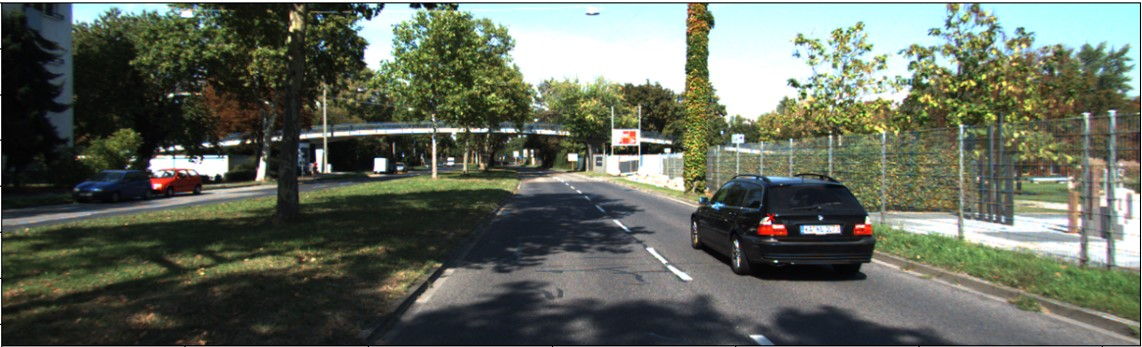
\includegraphics[width=\textwidth]{bb-fig1.jpg}
        \caption{Chosen center point}
        \label{fig:sfig-q3bb-cp}
    \end{subfigure}
    \begin{subfigure}[b]{\textwidth}
        \centering
        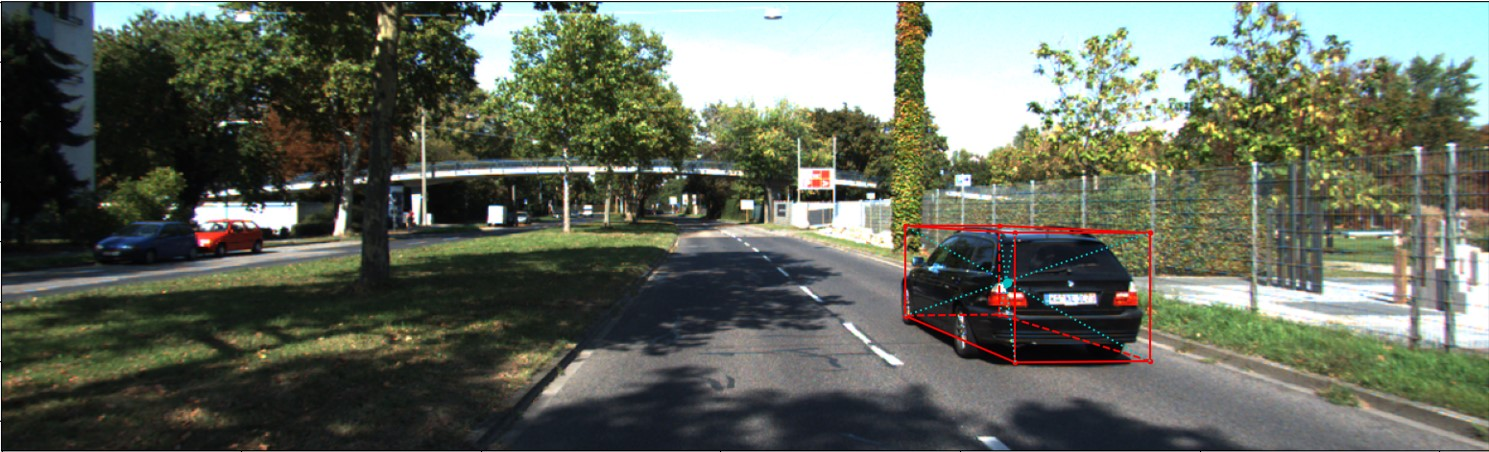
\includegraphics[width=\textwidth]{bb-fig2.jpg}
        \caption{Bounding box}
        \label{fig:sfig-q3bb-bb}
    \end{subfigure}
    \begin{subfigure}[b]{\textwidth}
        \centering
        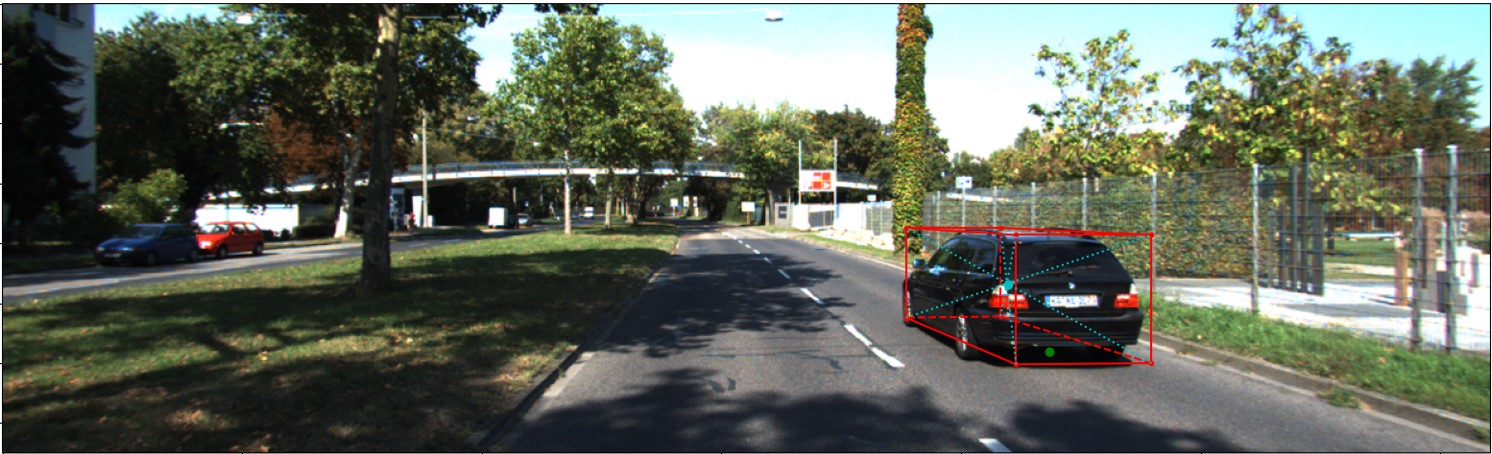
\includegraphics[width=\textwidth]{bb-fig3.jpg}
        \caption{Bounding box with the center of rear axle}
        \label{fig:sfig-q3bb-bbwca}
    \end{subfigure}
    \caption{Program output}
    \label{fig:q3-bb-output}
    \small
        In \ref{sub@fig:sfig-q3bb-cp}, the red cross is the center pixel

        In \ref{sub@fig:sfig-q3bb-bb}, the bounding box is shown

        In \ref{sub@fig:sfig-q3bb-bbwca}, the bounding box (in blue), along with the center of the rear axle (in green) is shown
\end{figure}

A part of the program output answering the question is shown below

\begin{displayquote}
    Center pixel is: 839, 234

    Vehicle BRD at (X, Y): 9.3510, -4.5330

    Rear axle in camera frame is (X, Y, Z): [ 3.70936019  1.65       10.10205256]

    Rear axle in image at (x, y): 874, 290    
\end{displayquote}
